\section{Примеры расчётов кровотока}
\subsection{Расчёт полной системы циркуляции}
Для примера применения одномерной модели кровотока для расчёта полной системы циркуляции рассмотрим
задачу о влиянии атеросклеротической бляшки на параметры течения крови, изученной в работе \cite{vassilevski:2011}.

На первом этапе решения задачи строится граф, описывающий изучаемую циркуляционную систему.
Он представленный двумя связанными сетями артерий и вен (см. Рис.~\ref{ss}). 
Сосудистая система состоит из 341 сосуда с анатомически адекватными свойствами (длина, диаметр, упругие свойства), вен и артерий. 
Вены и артерии соединены в 162 точках, на которые наложены граничные условия (\ref{eq:conserv-mass}),(\ref{eq:p-pressure}). 

\begin{figure}[h]
\centering
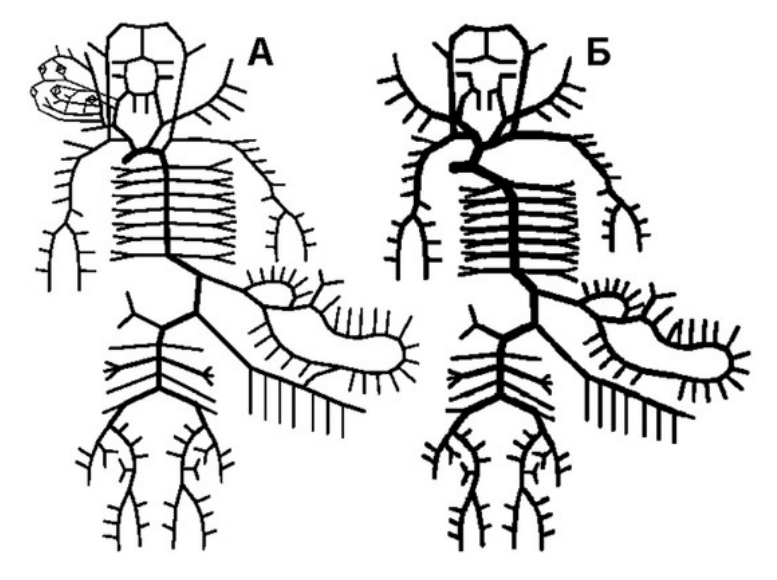
\includegraphics[width=0.5\linewidth]{krug.png}
\caption{Упрощённая структура сосудов системного круга. А—артерии, Б—вены.}
\label{ss}
\end{figure}

Далее в каждом сосуде вводится одномерную равномерную сетку и дискретизируем систему (\ref{eq:mass-balance}),(\ref{eq:momentum-balance}) 
методом монотонных характеристик первого порядка. Уравнения расширяются набором жестких ОДЕ, которые описывают работу сердца в терминах 
усредненной по объему модели.

Система жестких ОДУ, решаемая неявным методом Рунге-Кутта третьего порядка, обеспечивает граничные условия на входе и выходе сердца. 
Алгебраическая дифференциальная система (\ref{eq:mass-balance}),(\ref{eq:momentum-balance}), (\ref{eq:conserv-mass}),(\ref{eq:p-pressure}) 
в сочетании с зависимостью давления от площади и соответствующими граничными условиями на входе и выходе сердца 
и микроциркуляторных областях, решается по схеме с дробным шагом по времени схема, которая разделяет вычисления на 
локальные независимые части (отдельные сосуды и отдельные точки соединения).

На гиперболическом подэтапе применяется явный метод характеристик для каждого сосуда и контролируем шаг по времени с помощью 
ограничения устойчивости $\tau = 0.9 s_{\max}$, $s_{\max}=\max_{k,i}|\lambda _{k,i}|/h_k$, где $h_k$ -- размер сетки в сосуде $k$, 
$\lambda$ -- размер сетки в сосуде $k$,  $\lambda _{k,i}$ -- наибольшее (по величине) собственное значение якобиана для  (\ref{eq:mass-balance}),(\ref{eq:momentum-balance}), 
 в точке сетки.

В алгебраическом подэтапе применяется метод Ньютона для системы уравнений в каждом узле пересечения. 
Система состоит из уравнений (\ref{eq:conserv-mass}),(\ref{eq:p-pressure}) и условие совместимости по характеристикам (\ref{eq:mass-balance}),(\ref{eq:momentum-balance}). 
Влияние атеросклеротической бляшки учитывается в модели эластичной стенки. Здоровые сосуды описываются уравнением (\ref{eq:elastic-propeties}), 
обеспечивающим достоверную корреляцию с экспериментальными кривыми. Атеросклеротические артерии рассматриваются как 
трехслойные цилиндрические оболочки, деформированные внутренним давлением крови. Внутренний и внешний слои оболочки -- это 
фиброзная крышка и стенка артерии, соответственно. Деформации фиброзной пробки и стенки сосуда моделируются с помощью 
волоконно-эластичной модели. В простейшей версии волоконной осесимметричной модели оболочка представлена набором кольцевых волокон, 
которые сопротивляются только растяжению и сжатию волокон, как неогуковские материалы.

\begin{equation}
    \label{loc-force}
    \vec{F}=\frac{\partial}{\partial s}(T\vec{\tau}),
    \quad
    T=\mu\left(\left|\frac{\partial \vec{X}}{\partial s}\right|^2-\left|\frac{\partial \Vec{X}}{\partial s}\right|^{-2}\right).
\end{equation}
Здесь $\mathbf{F}$ обозначает плотность локальной силы, $T(s)$ обозначает натяжение волокна, 
$\Vec{\tau} =\partial \Vec{X}/\partial s^{-1}$ единичный касательный вектор, $\Vec{X}(s)$ 
представляет собой положение точек волокна в пространстве, координата Лагранжа s -- длина дуги волокна в ненапряженном состоянии. 
Липидный пул (промежуточная оболочка) имитируется набором радиальных пружин с нелинейной зависимостью между силой реакции и смещением

\begin{figure}[h]
\centering
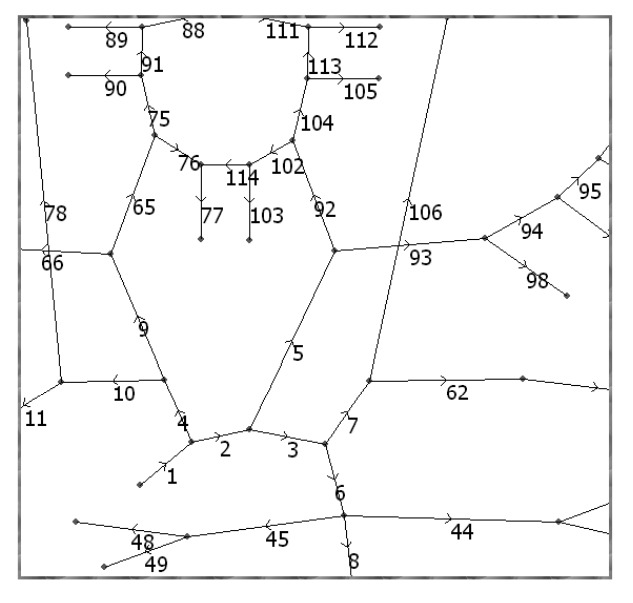
\includegraphics[width=0.4\linewidth]{chast.png}
\caption{Участок сосудов системного круга.}
\label{ych}
\end{figure}

\begin{figure}[h!]
\centering
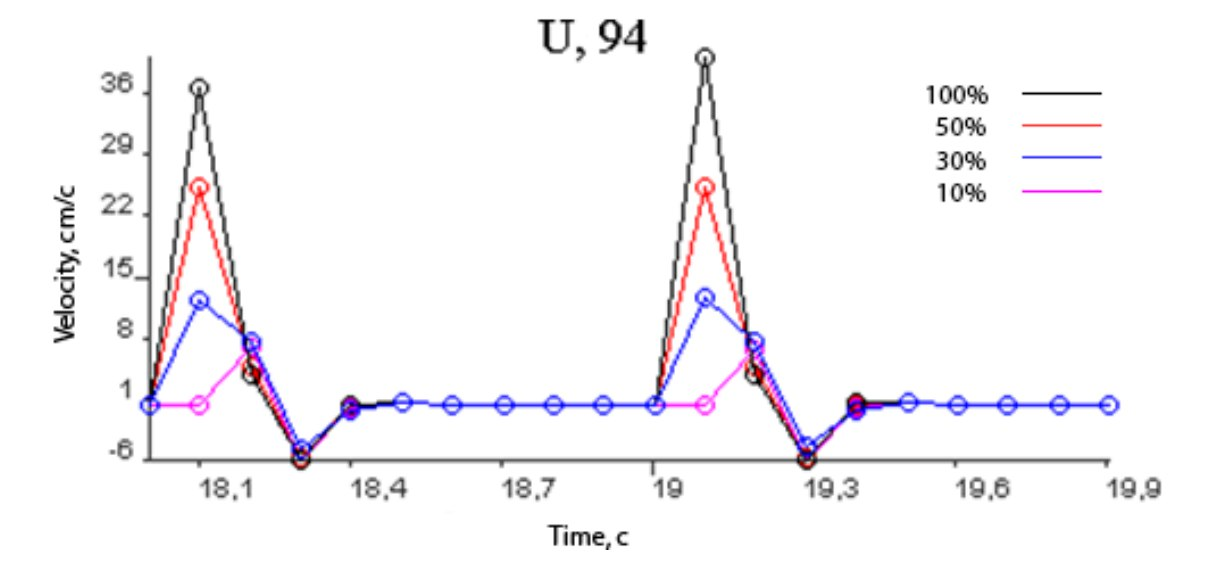
\includegraphics[width=0.45\linewidth]{94.jpg}
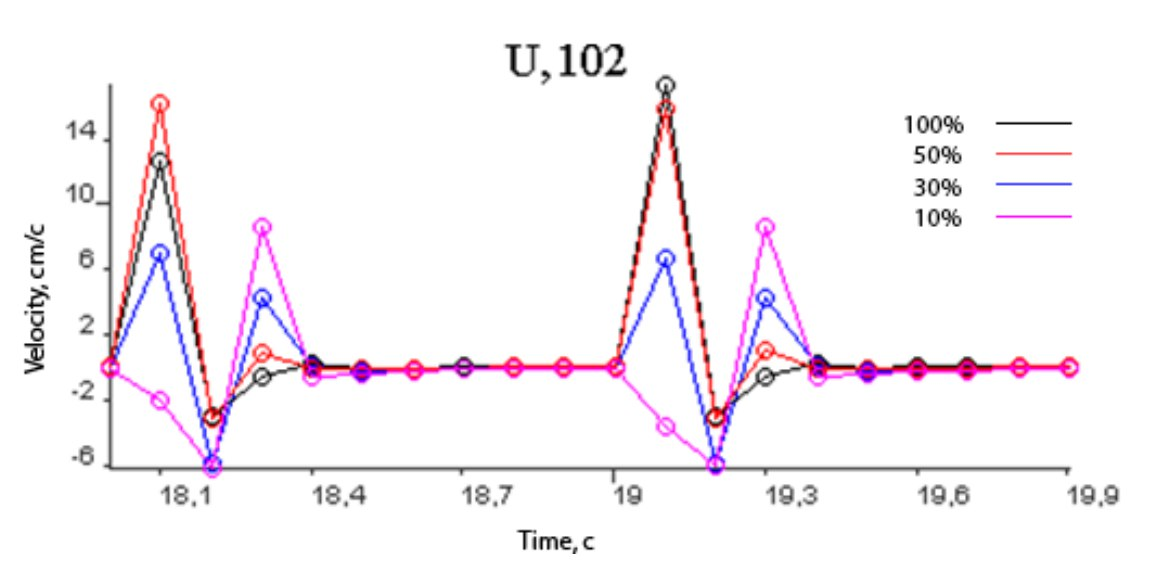
\includegraphics[width=0.45\linewidth]{102.jpg}\\
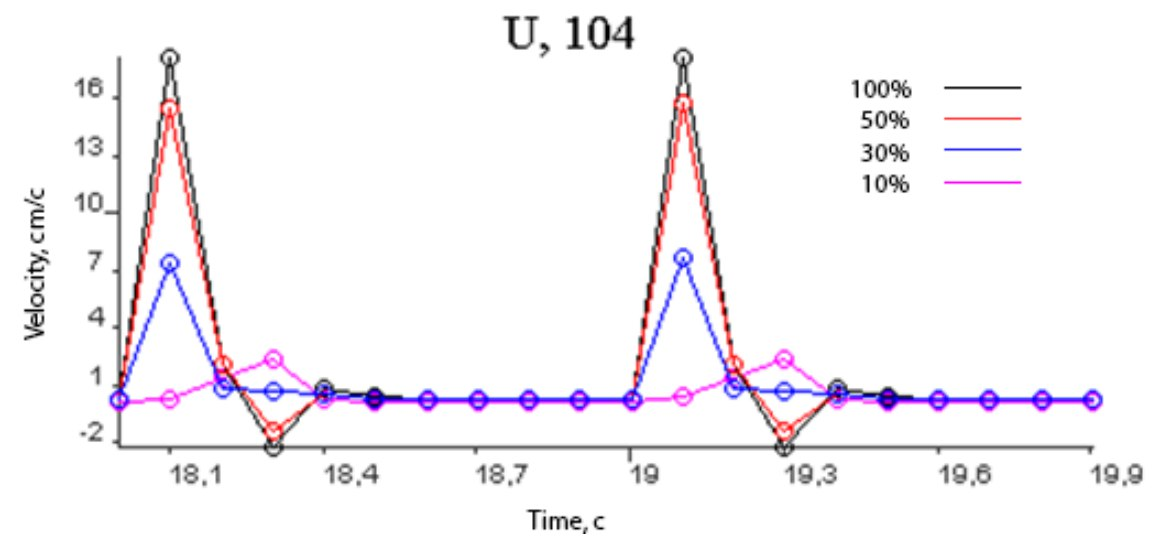
\includegraphics[width=0.45\linewidth]{104.jpg}
\caption{Скорость (см/с) в сосудах 94, 102, 104 для различных просветов. Здоровый сосуд
соответствует 100\% просвету}
\label{sc}
\end{figure}

Отношение давления к площади атеросклеротической артерии получено из предположения о статическом равновесии стенки: 
внутреннее давление крови уравновешивается упругими силами вышеупомянутой системы волоконных пружин, возникающими при ее смещении. 
На основе смещений можно рассчитать поперечную площадь сечения $A$ как реакцию на любое давление крови. 
Восстановление равновесного состояния получено в рамках его численной аппроксимации: конечно-разностная дискретизация (\ref{loc-force}) 
приводит к системе нелинейных алгебраических уравнений, которая должна быть решена итерационно методом Ньютона.

Численная модель <<волокно-пружина>> имеет преимущества прямые обобщения с другими типами волокон и, таким образом, 
может быть распространена на гораздо более широкий класс геометрий бляшек.

В численном эксперименте предполагается, что левая общая сонная артерия (№5 на Рис.\ref{ych}) повреждена протяженной атеросклеротической бляшкой 
с просветом 10\%, 30\%, 50\% и 100\%. Коэффициенты упругой бляшки взяты из~\cite{vassilevski:2011}. 
Профили скоростей в наружном сонном продолжении (№94) и артериях круга Виллиса (№104, 102) показаны на Рис.~\ref{sc}. 
Наиболее заметные изменения в скорости происходят в случае бляшек с просветом 30\% и 10\%. 
В малой артерии Виллисова круга (№104) и на продолжении левой наружной сонной артерии (№94) наблюдается значительное снижение скорости крови.


\subsection{Расчётная схема для моделирования течения в сосуде по одномерной модели}
Рассмотрим систему уравнений, описывающую кровоток в одиночном сосуде (\ref{eq:mass-conserv}) -- (\ref{eq:mom-conserv}) при условии
отсутствия источников/стоков ($\varphi=0$).
Из внешних сил, действующих на поток будем учитывать силу трения.
Для этого зададимся профилем скорости согласно \cite{smith:2002}:
$$
\tilde u(x, \xi) = u(x) \frac{\zeta + 2}{\zeta} \left[1 - \left(\frac{\xi}{r}\right)^\zeta\right],
$$
где $r$ -- радиус скругления, $\xi$ -- радиальная координата, $\zeta$ -- константа, определяющая профиль.
В результате интегрирования уравнений Навье-Стокса получим значение силы трения (см. \cite{boileau:2015}):

$$
\psi = -\frac{2 (\zeta + 2) \mu \pi u}{\rho A}.
$$

Запишем определяющую систему уравнений в виде

\begin{equation*}
    %\label{sys_of_eq}
    \begin{cases}
	&\dfrac{\partial A}{\partial t}+\dfrac{\partial Au}{\partial x}=0,\\[10pt]
	&\dfrac{\partial u}{\partial t}+u\dfrac{\partial u}{\partial x}+\dfrac{1}{\rho}\dfrac{\partial p}{\partial x}=\psi(u, A),\\[10pt]
	&p=\dfrac{4}{3}\sqrt{\pi}\dfrac{Eh}{A_0}(\sqrt{A}-\sqrt{A_0}).
    \end{cases}
\end{equation*}
Здесь использована замыкающая зависимость $p(A)$ из работы \cite{boileau:2015}, учитывающая
эластичные свойства стенок сосудов через параметры $E$ -- модуль упругости и $h$ -- толщина стенок сосуда.

Проведём обезразмеривание системы:
\begin{equation}
    \label{sys_of_eq1}
    \begin{cases}
	\dfrac{\partial A}{\partial t}+\dfrac{\partial Au}{\partial x}=0,\\[10pt]
	\dfrac{\partial u}{\partial t}+\dfrac{1}{2}\dfrac{\partial u^2}{\partial x} = -\dfrac{\partial p}{\partial x}-M_f \dfrac{u}{A},\\[10pt]
	p=M_p(\sqrt{A}-1).
    \end{cases}
    \end{equation}
В результате все физические параметры задачи определены через два безразмерных комплекса
$$
M_f=\frac{2(\zeta+2)\mu \pi L}{\rho A_0 U_0}, \quad
M_p=\frac{4\sqrt{\pi}Eh}{3 \rho U_0^2\sqrt{A_0}},
$$
где $L$ -- характерная длина сосуда, $A_0$ -- характерная площадь поперечного сечения сосуда, $U_0$ -- характерная скорость потока.
Первое из них описывает трение жидкости о стенки сосуда, второе -- эластичные свойства стенок сосуда.
Характерное время процесса при этом определится как $t_0 = L/U_0$.

Определяющая система дифференциальных уравнений (\ref{sys_of_eq1}) включает в себя два гиперболических уравнения.
Первое из них имеет вид уравнения переноса, второе -- уравнения Бюргерса.

{\bf Дискретизация по времени.}
Запишем входящие в систему (\ref{sys_of_eq1}) дифференциальные уравнения
в общем виде:
\begin{equation}
\label{eq:hyper}
\dfrac{\partial f}{\partial t}+\dfrac{\partial F(u, f)}{\partial x} = S(u, f).
\end{equation}
Для дискретизации по времени будем использовать явную схему c шагом $\tau$:
$$
\frac{\hat f - f}{\tau} + \frac{\partial F(u, f)}{\partial x} = S(u, f).
$$

{\bf Аппроксимация по пространству. TVD-схема.}
Известно, что пространственная аппроксимация гиперболического слагаемого схемой второго порядка точности неустойчива,
а использование схемы первого порядка (схемы против потока) приводит к большому влиянию численной диффузии на решение.
Для построение низкодиссипативной устройчивой схемы будем использовать метод TVD \cite{mazo1:2018},
которая заключается в комбинировании схем первого и второго порядка в зависимости от значения градиента искомой функции.

Запишем уравнение (\ref{eq:hyper}) в полудискретизованном с шагом $h$ виде в $i$-том узле расчётной сетки:
$$
\dfrac{\partial f_i}{\partial t}+\dfrac{F_{i + 1/2} - F_{i - 1/2}}{h} = S_i(u, f).
$$

Значение потока вычисленные по схеме первого и второго порядка точности определятся в виде
$$
\begin{aligned}
	&F^u_{i+1/2}=\begin{cases}
		F_i, &u_i>0\\
		F_{i+1},& u_i<0
	\end{cases}\\[10pt]
	&F^h_{i+1/2}=\dfrac{F_i + F_{i+1}}{2}.
\end{aligned}
$$

А само значение $F$ запишется в виде
$$
F_{i+1/2} = F^u_{i+1/2} + \phi(r) \left(F^h_{i+1/2} - F^u_{i+1/2}\right),
$$
где $\phi$ -- функция-ограничитель, а $r$ -- определяется через сеточный градиент искомой функции
$$
r = \frac{f_i - f_{i-1}}{f_{i+1} - f_{i}}.
$$
\clearpage
{\bf Тестовая задача о бегущей волне} -- классическая задача для тестирования схем аппроксимации гиперболических уравнений.
Постановка задачи имеет вид
\begin{equation*}
\dfrac{\partial f(x, t)}{\partial t}+\dfrac{\partial f(x, t)}{\partial x} = 0
\end{equation*}
и начальные условия
$$
f(x, 0) = \begin{cases}
	1, \quad \left|x\right| \leq 0.2,\\
	0, \quad \left|x\right| > 0.2.
\end{cases}
$$


Для тестирование схемы рассматривались ограничители вида 

Upwind: $ \phi(r)=0 $

MinMod: $
\begin{aligned}
	\phi(r)=\begin{cases}
	0, &r\leq 0\\
	r, &0<r\leq 1\\
	1, &r>1
    \end{cases}
\end{aligned}
$


MC: $
\begin{aligned}
     \phi(r)=\begin{cases}
	0, &r\leq0\\
	2r, &0<r\leq\frac{1}{3}\\
	\frac{1+r}{2}, &r\leq3\\
	2, &r>3
    \end{cases}
\end{aligned}
$ 


VanLeer:$
\begin{aligned}
    \phi(r)=\frac{r+|r|}{1+|r|}
\end{aligned}
$


SuperBee: $
\begin{aligned}
    \phi(r)=\begin{cases}
	0, &r\leq 0\\
	2r, &0<r\leq 0.5\\
	1, &0.5<r\leq 1\\
	r, &1<r\leq 2\\
	2, &r>2
    \end{cases}
\end{aligned}
$


Umist: $
\begin{aligned}
    \phi(r)=\begin{cases}
	0, &r\leq 0\\
	2r, &0<r\leq 0.2\\
	0.52+0.75r, &0.2<r\leq \frac{3}{7}\\
	0.75+0.25r, &\frac{3}{7}<r\leq \frac{7}{3}\\
	2, &r>\frac{7}{3}
    \end{cases}
\end{aligned}
$


Ospre: $
\begin{aligned}
   \phi(r)=
    \frac{1.5(r^2+r)}{r^2+r+1}
\end{aligned}
$


На основе описанного выше можно произвести расчёты и построить графики распределения объема по времени, а так же сравнить
заданные ограничители.
Задача решалась с шагом по пространству $h=1/30$ и шагом по времени $\tau=0.007$.

\begin{figure}[h!]
    \centering
    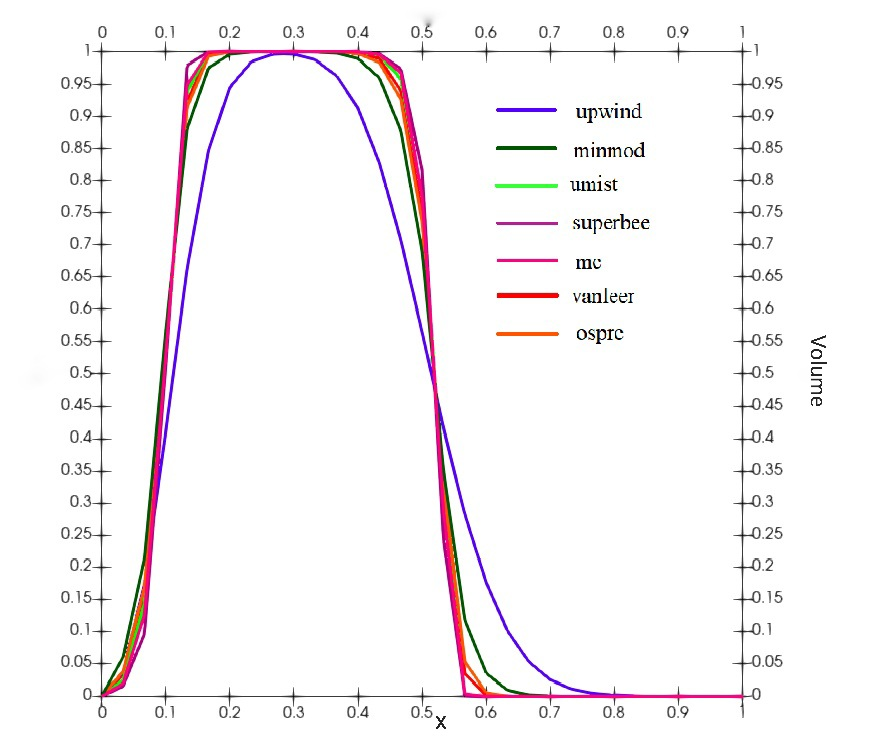
\includegraphics[width=0.6\linewidth]{03.jpeg}
    \caption{Распределение объёма в момент 0.3}
    \label{03}
\end{figure}

\begin{figure}[h!]
    \centering
     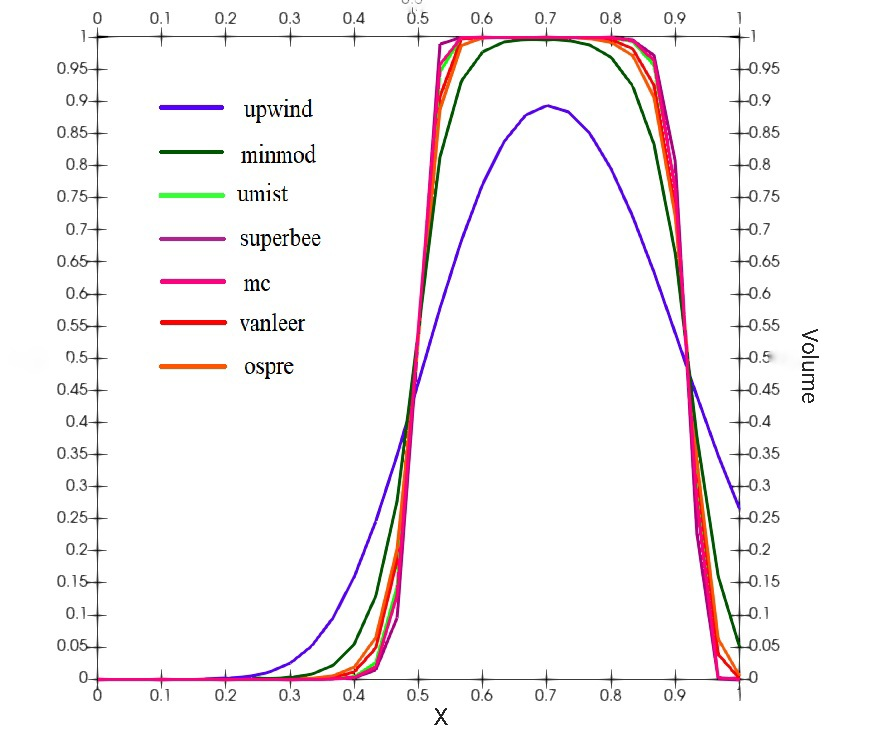
\includegraphics[width=0.6\linewidth]{07.jpeg}
    \caption{Распределение объёма в момент 0.7}
    \label{07}
\end{figure}


\begin{figure}[h!]
    \centering
     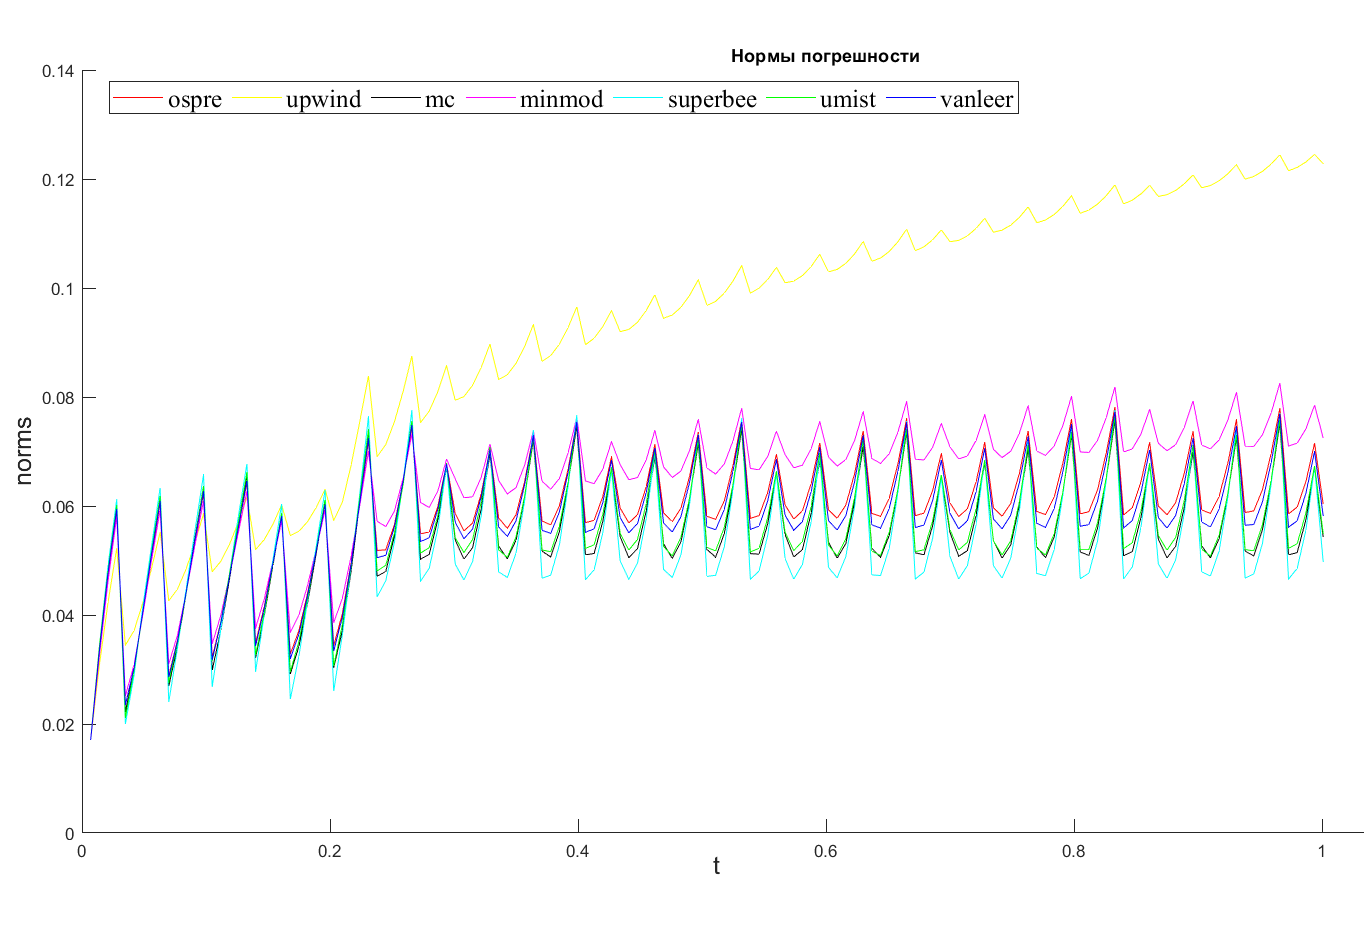
\includegraphics[width=1\linewidth]{norm.png}
    \caption{График погрешностей.}
    \label{norms}
\end{figure}

\begin{table}[h]
\centering
\caption {Значения погрешностей в момент 0.56 численного решения уравнения переноса}
\label{tab:norms_transport}
\begin{tabular}{|l|l|c|c|c|c|c|c|c|c|}
\hline
Ограничитель & Значение \\
\hline
SuperBee & 0.0659053\\
\hline
MC &  0.0659238\\
\hline
Umist & 0.0663728\\
\hline
Van Leer & 0.0685166\\
\hline
Ospre &  0.069493\\
\hline
MinMod & 0.0737164\\
\hline
Upwind  & 0.103783\\
\hline
\end{tabular}
\end{table}


На основе полученных данных можем сделать вывод, что для моделирования данной задачи не стоит использовать такие ограничители, как
Upwind и MinMod, а самыми точными оказались SuperBee и MC.
\clearpage
{\bf Тестовая задача: уравнение Бюргерса.} Рассмотрим уравнение вида
$$
\dfrac{\partial u(x, t)}{\partial t}+\dfrac12\dfrac{\partial u^2(x, t)}{\partial x} = 0
$$
с начальными условиями
$$
u(x, 0) = \begin{cases}
	1 - (x-1)^2, \quad \left|x-1\right| \leq 1,\\
	0, \quad \left|x-1\right| > 1.
\end{cases}
$$
Точное решением этой задачи на моменты времени $t<0.5$ будет иметь вид
$$
u_e = 1-\frac{{{\left( 1-\sqrt{1+4 t\, \left( t-x+1\right) }\right) }^{2}}}{4 {{t}^{2}}}
$$

Задача решалась с шагом по пространству  $h=0.1$ и шагом по времени $\tau=0.025$.
На рисунке \ref{fig:burgers} и в таблице \ref{tab:burgers} представлены решения и среднеквадратичные отклонения, полученные с использованием различных ограничителей.
Также как и в случае с задачей о бегущей волне, наиболее близкие к точному решению удалось получить с использованием ограничителя Superbee.

\begin{figure}[h]
\centering
\includegraphics[width=0.5\linewidth]{burgers.png}
\caption{Сравнение численного и точного решений уравнения Бюргерса на момент $t=0.5$}
\label{fig:burgers}
\end{figure}

\begin{table}[h]
\centering
\caption {Значения погрешностей в момент $t=0.5$ численного решения уравнения Бюргерса}
\label{tab:norms_burgers}
\begin{tabular}{|l|l|}
\hline
Ограничитель & Значение \\
\hline
SuperBee & 0.025357\\
\hline
Van Leer & 0.0279678\\
\hline
Upwind  & 0.050419\\
\hline
\end{tabular}
\end{table}

\clearpage
{\bf Тестовая задача: задача об одиночном импульсе.}
Рассмотрим задачу (\ref{sys_of_eq1}) о течении в канале с физическими параметрами, представленными в 
таблице \ref{tab:single_impulse_params}.

\begin{table}[h]
\centering
\caption {Параметры задачи об одиночном импульсе}
\label{tab:single_impulse_params}
\begin{tabular}{|l|l|}
\hline
$L$ & 2 м \\
\hline
$A_0$ & $\pi$ см$^2$\\
\hline
$h$ & $1.5$ мм\\
\hline
$\rho$  & 1050 кг/м$^3$\\
\hline
$\mu$  & 0 или 4 мПа$\cdot$с\\
\hline
$\zeta$  & 9\\
\hline
$E$  & 4$\cdot10^5$ Па\\
\hline
\end{tabular}
\end{table}

В качестве входного расхода используем функцию
$$
Q(t) = 10^{-6} \exp\left(-10^{-4}(t-0.05)^2\right) \quad m^3/s
$$
имеющую вид импульса с максимальным значением $10^{-6}$ м$^3$/с в момент времени $t=0.05$ сек.

В результате обезразмерирования получим следующие значения безразмерных комплексов, входящих в определяющую систему
$$
M_f = 0 \text{ или } 263.295,\quad  M_p = 7.5\cdot10^{6}.
$$

Задача решалась с шагом по пространству $h=5\cdot10^{-4}$ и шагом по времени $\tau=2 \cdot 10^{-5}$.
Численное решение на момент времени $t=10^{-3}$ представлено на рисунке \ref{fig:single_pulse_result}.

\begin{figure}[h]
\centering
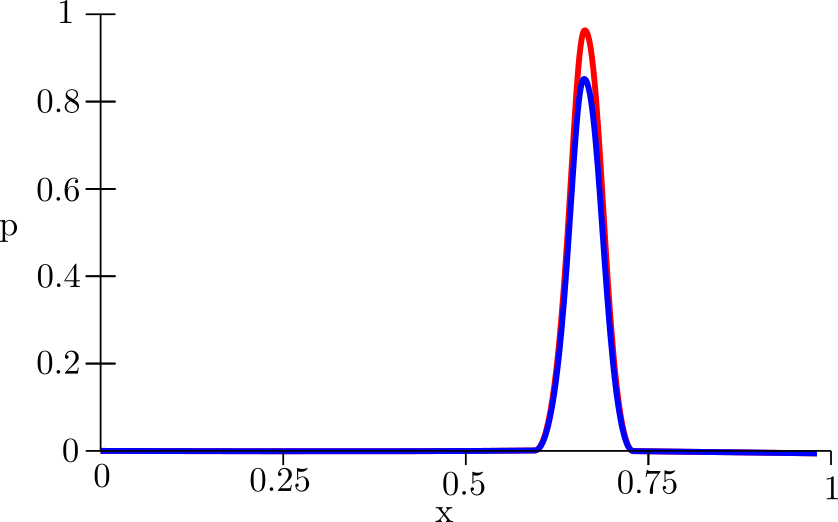
\includegraphics[width=0.5\linewidth]{single_pulse.png}
\caption{Значение давления для задачи одиночного импульса на момент $t=10^{-3}$. Красная линия соответствует параметру $M_f=0$, синяя -- $M_f=263.295$}
\label{fig:single_pulse_result}
\end{figure}
